\lhead[\thepage]{CAPÍTULO \thechapter. DISEÑO}
\chead[]{}
\rhead[WepSIM: Simulador de un procesador elemental con unidad de control microprogramada\leftmark]{\thepage}
\renewcommand{\headrulewidth}{0.5pt}

\lfoot[]{}
\cfoot[]{}
\rfoot[]{}
\renewcommand{\footrulewidth}{0pt}

%% This is an example first chapter.  You should put chapter/appendix that you
%% write into a separate file, and add a line \include{yourfilename} to
%% main.tex, where `yourfilename.tex' is the name of the chapter/appendix file.
%% You can process specific files by typing their names in at the 
%% \files=
%% prompt when you run the file main.tex through LaTeX.
\chapter{Diseño}
\label{ch:design}
\markboth{}{DESIGN}

En este capítulo se realiza una descripción completa del simulador desarrollado, incluyendo la arquitectura interna y los diferentes módulos \gls{software}, que componen la herramienta descritos con anterioridad en \cite{mateos2016wepsim}.

La Sección \ref{sec:study_of_solution} discute el estudio de la solución final, considerando las diferentes alternativas existentes para el diseño y desarrollo del simulador. En la Sección \ref{sec:solution_selection} se indica la solución elegida y la compara con las alternativas consideradas. La Sección \ref{sec:simulator_architecture} describe cada uno de los módulos que componen el simulador.

\section{Estudio de la solución final}
\label{sec:study_of_solution}

Debido a los requisitos de usuario establecidos en este proyecto (Sección \ref{sec:user_requirements}), en donde se especificaba que el \gls{software} no debía ser instalado en el dispositivo del usuario, y debía de poder ser ejecutado en los navegadores web indicados, se ha decidido que el diseño del simulador esté enfocado como una aplicación web.

Existen diferentes modelos arquitectónicos a la hora de realizar el diseño de una aplicación web. La primera opción, es el modelo cliente-servidor en el cual las tareas se reparten entre dos roles: un proveedor que proporciona recursos o servicios que es llamado servidor, y un consumidor que contacta con el servidor con el objetivo de hacer uso de los recursos que éste provee. Es un modelo distribuido en el que la lógica de negocio y el cómputo recaen en el servidor, y el cliente provee la interfaz de usuario, realizando validaciones y procesos menores de la lógica de negocio. La segunda opción, es un modelo en el que toda la aplicación es ejecutada en el cliente, siendo únicamente necesario el servidor para el acceso al código de la aplicación. Este modelo, posibilita incluso que el servidor no sea necesario en el caso de existir el código de la aplicación web en el cliente, pudiendo ser ejecutada sin la necesidad de internet. Ambos modelos son independientes del sistema operativo sobre el que la aplicación  se ejecuta y dependen exclusivamente del soporte del navegador, dotando a la aplicación de compatibilidad con un amplio abanico de plataformas.

Debido a los requisitos de usuario establecidos en este proyecto (Sección \ref{sec:user_requirements}), la segunda opción es la que cumple con la necesidad de no necesitar acceso a internet, de forma que la funcionalidad total del simulador quede en el dispositivo del usuario.

Una vez decidido el modelo de diseño, es necesario tener en cuenta las diferentes tecnologías a utilizar. Como se indicó en la sección \ref{sec:user_requirements}, es necesario que la aplicación sea diseñada siguiendo el lenguaje de marcado \acrshort{html}5, que está formado por \acrshort{html}, \acrshort{css} y JavaScript. De este modo, es necesario contemplar los diferentes frameworks y bibliotecas existentes que ayudan a la hora de realizar el diseño de la aplicación, posibilitando el funcionamiento de ésta tanto en ordenadores como en dispositivos móviles. Estas tecnologías descritas anteriormente en la Sección \ref{sec:tecnologias_web}, proporcionan distintas funcionalidades y enfoques a la hora de diseñar la aplicación, permitiendo la compatibilidad de la aplicación con la amplia mayoría de los navegadores web. En la Tabla \ref{tab:comparison_webframeworks}, se analizan las funcionalidades y compatibilidades que proporcionan estas tecnologías, valorando si cumplen con los requisitos establecidos en este proyecto.

\begin{table}[htbp]
\ra{1.2}
\centering
\caption{Comparación de frameworks y bibliotecas.}
%\resizebox{\textwidth}{%
\resizebox{\textwidth}{!}{
\begin{tabular}{@{}llllllll@{}}
\toprule
\textbf{Framework} & \textbf{Angular.js} & \textbf{jQuery.js} & \textbf{BootStrap} & \textbf{Dojo} \\ 
\midrule
Funcionalidad requerida			& \ding{51}  &  \ding{51} & \ding{51} & \ding{51} \\
\midrule
Ejecución en cliente				& \ding{51} & \ding{51} & \ding{51} &  \\
\midrule
Compatibilidad navegadores requeridos				& \ding{51} & \ding{51} & \ding{51} & \ding{51} \\
\midrule
Soporte plataformas móviles				& \ding{51}  & \ding{51}  & \ding{51}  & \\
\bottomrule
\end{tabular}
}
\label{tab:comparison_webframeworks}
\end{table}

De este modo,  pese a que \textit{Angular.js} nos proporciona la mayoría de funcionalidades requeridas, tiene una curva de aprendizaje bastante mayor que \textit{jQuery}, lo cual hace que \textit{jQuery} se imponga a la hora de su elección debido a que las ventajas que supondría utilizar \textit{Angular.js} quedan disueltas por este inconveniente. Por otro lado, sería interesante el uso de \textit{Dojo} a la hora de utilizar una tecnología que nos proporcione funcionalidad y efectos en la interfaz de usuario y nos ayude a la capturación de eventos, pero queda descartado al estar enfocado a aplicaciones que utilizan \acrshort{ajax}. De esta forma, \textit{BootStrap} será la tecnología elegida para dotar a la aplicación de la funcionalidad requerida a nivel de interfaz de usuario y complementando tanto a JavaScript como a jQuery.

\subsection{Solución elegida}
\label{sec:solution_selection}

Para que los profesores de la asignatura Estructura de Computadores puedan hacer uso de una herramienta que sirva de ayuda para la explicación de los conceptos teóricos de la asignatura, y los estudiantes puedan utilizarla para comprender estos conceptos y realizar posteriormente las prácticas de la asignatura, se propone el diseño e implementación de una herramienta web que simule con realismo en funcionamiento de un procesador elemental con unidad de control microprogramable.

Este simulador, será desarrollado como una herramienta web debido a la portabilidad que proporciona, ya que podrá ser ejecutado sobre un gran número de diferentes dispositivos independientemente del sistema operativo que utilice, puesto que únicamente necesita un navegador web para su correcto funcionamiento. De esta forma, los profesores y estudiantes podrán hacer uso de la herramienta sin depender de su instalación en el dispositivo a utilizar, incluso pudiendo los estudiantes realizar las prácticas sobre dispositivos móviles.

Para lograr dicha portabilidad, el simulador ha sido desarrollado en \acrshort{html}5 (\acrshort{html} + JavaScript + \acrshort{css}) haciendo posible su ejecución en cualquier plataforma \emph{(smartphones, tablets, \acrshort{pc}s, etc.)} que pueden ejecutar Microsoft Edge, Mozilla Firefox, Google Chrome o Safari. Además, la herramienta depende de los siguientes frameworks/bibliotecas: JQuery, JQueryUI, JQuery Mobile, Knockout y BootStrap.

Por tanto, la solución elegida es capaz de unificar en una misma herramienta todas las funcionalidades requeridas para la enseñanza de Estructura de computadores con un alto nivel de detalle, con alta disponibilidad al facilitarse su como una herramienta web, y con una gran portabilidad puesto que podrá ser ejecutada sobre un gran número de diversos dispositivos, buscando en todo momento una solución sin la necesidad de servidor.

\section{Arquitectura de \acrshort{wepsim}}
\label{sec:simulator_architecture}

La arquitectura de la solución presentada en este trabajo consta de tres elementos principales:

\begin{itemize}
\item \textbf{Modelo \gls{hardware}:} permite definir el \gls{hardware} a usar.
\item \textbf{Modelo \gls{software}:} permite definir el juego de instrucciones a utilizar.
\item \textbf{Kernel de simulación:} simula el funcionamiento del \gls{hardware} ejecutando el \gls{microcodigo}/lenguaje máquina definido con anterioridad.
\end{itemize}

El modelo \gls{hardware} permite definir los distintos elementos típicos de un computador (memoria principal, procesador, etc.) de una forma modular. La forma de definir estos elementos equilibra dos objetivos contrapuestos: es suficientemente completa como para imitar los principales aspectos de la realidad, pero es lo suficientemente mínima para facilitar su uso. Ante todo se persigue que sea una herramienta didáctica.

El modelo \gls{software} permite definir el \gls{microcodigo} y el \gls{ensamblador} basado en este \gls{microcodigo} de la forma más intuitiva posible. El \gls{ensamblador} a usar viene dado por un conjunto de instrucciones que puede ser definido por el usuario e intenta ser lo suficientemente flexible como para poder definir diferentes tipos y juegos de instrucciones, como por ejemplo MIPS o ARM.

El tercer elemento de la arquitectura propuesta es un kernel que toma como entrada el modelo \gls{hardware} descrito y el modelo \gls{software} de trabajo, y se encarga de mostrar el funcionamiento del \gls{hardware} con el \gls{software} dado.

\begin{figure}[htbp]
 	\centering
 	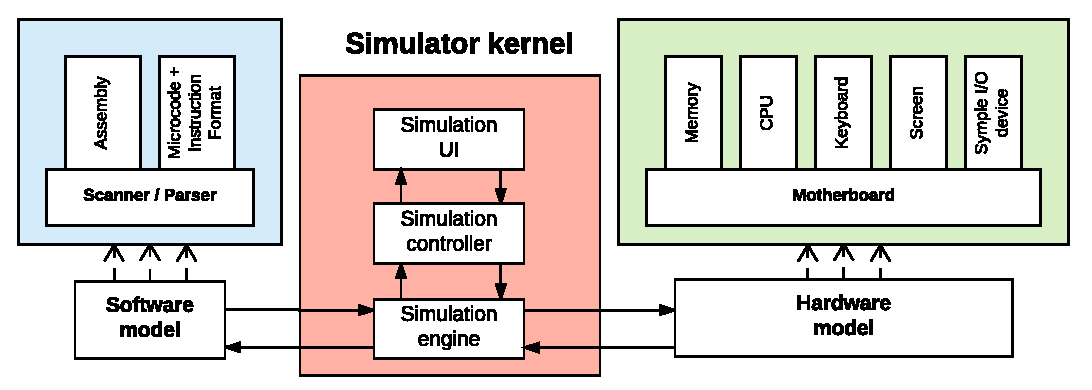
\includegraphics[width=14cm]{figures/architecture_diagram}
 	\caption{Arquitectura de \acrshort{wepsim}.}
	\label{fig:architecture_diagram}
\end{figure}

La Figura \ref{fig:architecture_diagram} resume la arquitectura de \acrshort{wepsim}. El punto de inicio es el modelo \gls{hardware} que describe el procesador a ser simulado. Esto incluye el procesador, la memoria y algunos dispositivos de E/S: teclado, pantalla y un dispositivo de E/S simple que genera interrupciones. El modelo \gls{hardware} describe el estado global del procesador. A partir del estado global del procesador, el kernel de simulación actualiza el estado en cada ciclo de reloj.

La unidad de control simulada almacena las señales de control de cada ciclo en una memoria de control. La memoria de control tiene todos los microprogramas para las instrucciones con las que trabaja el procesador, y el fetch para leer la instrucción de memoria y decodificarla.


El \gls{microcodigo} (el contenido de la memoria de control) junto con el formato de cada instrucción (campos de la instrucción y su longitud) se describe en un fichero de texto. El modelo \gls{software} lee este fichero, lo traduce a binario y lo carga en el procesador. La definición del lenguaje \gls{ensamblador} a utilizar se describe junto con el \gls{microcodigo}, y el modelo \gls{software} permite traducir a binario programas escritos en dicho \gls{ensamblador}.


El kernel de simulación pregunta al subsistema del modelo \gls{software} por el \gls{microcodigo} definido, la descripción del formato de instrucción y el contenido de la memoria principal. Los binarios se cargan en los elementos del modelo \gls{hardware}, y a continuación el kernel de simulación actualiza el estado global en cada ciclo de reloj.


\acrshort{wepsim} dispone de un controlador de simulación que se encarga de actualizar el ciclo de reloj y mostrar el estado global. El subsistema de interfaz de simulación actualiza la interfaz de usuario. Cuando el usuario usa la interfaz de usuario para solicitar una operación, el subsistema de interfaz de simulación traslada la petición al controlador de simulación. De este modo, se usa un Modelo- Vista-Controlador (MVC) básico para la arquitectura de \acrshort{wepsim}.

\subsection{Modelo \gls{hardware}}

El modelo \gls{hardware} que usa \acrshort{wepsim} permite definir los distintos elementos típicos de un computador (memoria principal, procesador, etc.) de una forma modular y de manera que sea posible añadir, quitar o modificar estos elementos.

\begin{figure}[htbp]
 	\centering
 	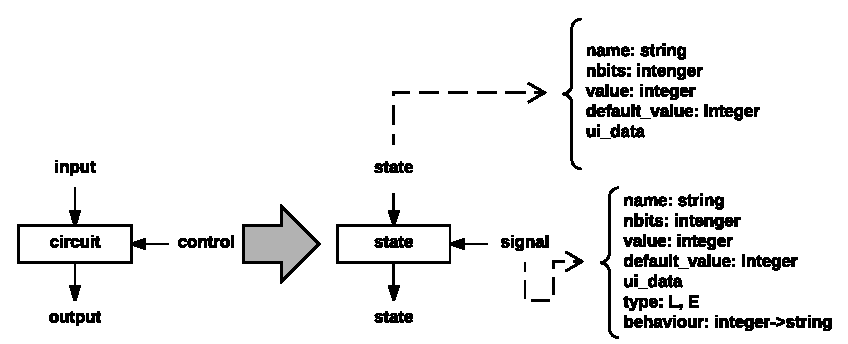
\includegraphics[width=14cm]{figures/hardware_model}
 	\caption{Modelado del \gls{hardware}.}
	\label{fig:hardware_model_diagram}
\end{figure}

La figura \ref{fig:hardware_model_diagram} introduce el modelo propuesto. Cada elemento del circuito se describe como una caja negra con posibles entradas, posibles salidas y señales de control (que controlan las posibles transformaciones de las entradas a las salidas). El subsistema del modelo \gls{hardware} transforma esta caja negra en dos conjuntos de objetos: estados y señales. Un estado tiene un identificador (el nombre), el valor (un valor entero) y un valor inicial (el valor por defecto). Los valores que puede tomar son valores naturales dentro de un rango, dado por el número de bits con los que se representa el estado. Una señal es un estado especial que controla el valor de otros estados o señales. Hay dos atributos asociados a las señales (y no a los estados): el tipo de señal (por nivel o por flanco) y su comportamiento. Para cada valor de señal una cadena de caracteres describe en un lenguaje simple lo que la señal mueve o transforma. Este lenguaje simple se compone principalmente de instrucciones que representan las operaciones elementales.

\begin{figure}[htbp]
 	\centering
 	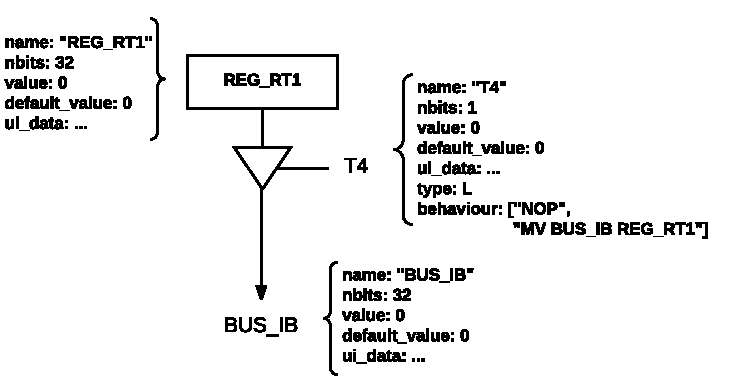
\includegraphics[width=14cm]{figures/hardware_example_tristate}
 	\caption{Ejemplo de modelado de una puerta triestado.}
	\label{fig:hardware_tristate_example}
\end{figure}

\begin{figure}[htbp]
 	\centering
 	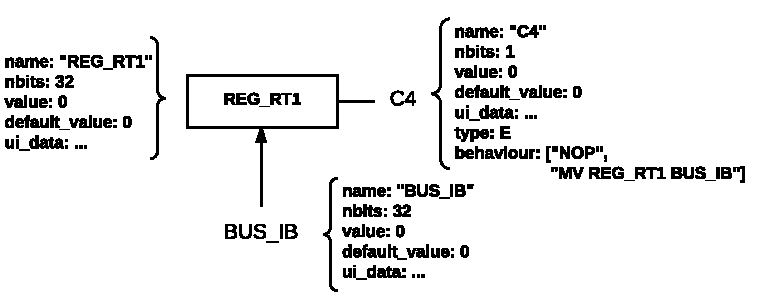
\includegraphics[width=14cm]{figures/hardware_example_register}
 	\caption{Ejemplo de modelado de un registro.}
	\label{fig:hardware_register_example}
\end{figure}

Las Figuras \ref{fig:hardware_tristate_example} y \ref{fig:hardware_register_example} muestran dos ejemplos: un triestado y un registro.
El triestado controla dos estados: el estado del bus al que se conecta \emph{BUS IB} y el estado del registro de entrada, \emph{REG RT1} en este caso. Ambos representan el valor a la salida de la puerta (\emph{BUS IB}) y el valor del registro \emph{RT1 (REG RT1)}. La señal \emph{T4} se encarga de indicar cuándo el valor del registro \emph{RT1} se envía a la salida. Esta señal \emph{T4} es una señal por nivel (tipo: L), con valor cero no tiene efecto (comportamiento ``NOP''). Cuando el valor de la señal es uno entonces el comportamiento es el de copiar el valor del registro \emph{RT1} a la salida (comportamiento \emph{``MV BUS IB REG RT1''}).

El ejemplo con el registro (Figura \ref{fig:hardware_register_example}) es similar. En este caso se trabaja con dos estados: el contenido del registro \emph{RT1} y el contenido situado a la entrada (\emph{BUS IB}). La señal \emph{C4} controla cuándo se almacena en el registro \emph{RT1} el valor que hay en la entrada. La diferencia está en el tipo de señal: \emph{C4} es una señal por flanco de bajada (tipo: E), por lo que al final del ciclo de reloj (pasa de uno a cero) si la señal vale uno entonces el comportamiento es el de copiar el valor situado a la entrada al registro (comportamiento \emph{``MV REG RT1 BUS IB''}).

El lenguaje simple usado para definir los comportamientos añade a las operaciones elementales otras operaciones necesarias. Por ejemplo disparar una señal (\emph{``FIRE C4''}) que ayuda a propagar el efecto de una señal al re-evaluar la señal inmediata que podría verse afectada. Otro ejemplo lo encontramos en dos operaciones que pueden ser muy útiles a la hora de depurar: imprimir el valor de un estado (\emph{``PRINT E BUS IB''}) e imprimir el valor de una señal (\emph{``PRINT S C4''}).

\subsection{Modelo \gls{software}}

Una vez definido el procesador elemental usando el modelo \gls{hardware} propuesto, es necesario describir el conjunto de instrucciones que es capaz de ejecutar así como el \gls{microcodigo} que lo orquesta. En un fichero de texto se define el formato de las instrucciones máquina junto con el cronograma asociado a la ejecución de cada una de las instrucciones máquina. La Figura \ref{fig:software_format_example} muestra un ejemplo de definición para la instrucción \emph{li (load inmmediate)}, que almacena un valor inmediato en un registro.

\begin{figure}[htbp]
 	\centering
 	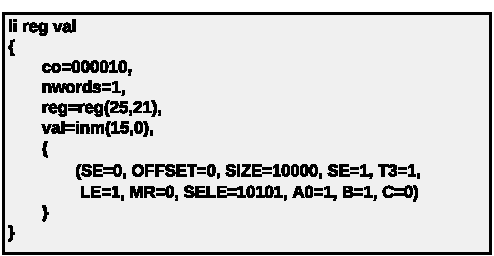
\includegraphics[width=10cm]{figures/instruction_example}
 	\caption{Ejemplo de formato de instrucción.}
	\label{fig:software_format_example}
\end{figure}

\vspace{10mm}

El fichero con el cronograma de fetch y todos los cronogramas de las instrucciones define el \gls{microcodigo} para la plataforma \acrshort{wepsim}. El simulador permite la definición de diferentes juegos y formatos de instrucciones. Inicialmente se ha implementado un subconjunto de las instrucciones del MIPS, pero es posible definir instrucciones de otros conjuntos de forma similar. En este fichero se pueden asignar códigos simbólicos a los registros del banco de registros, lo que permite que en los programas escritos en \gls{ensamblador} se puedan usar dichos  símbolos (por ejemplo, registro \emph{\$t3} en la Figura \ref{fig:software_assembly_example}).

\begin{figure}[htbp]
 	\centering
 	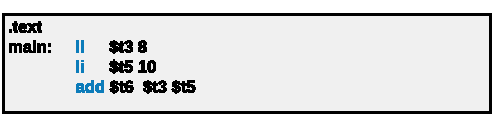
\includegraphics[width=10cm]{figures/example_assembly}
 	\caption{Ejemplo de código fuente en \gls{ensamblador}.}
	\label{fig:software_assembly_example}
\end{figure}

El campo \emph{``co''} identifica el código de instrucción máquina, que es un número binario de 6 bits. Esto permite definir hasta 64 instrucciones distintas. Dado que los últimos 4 bits de la instrucción pueden usarse para seleccionar la operación en la \acrshort{alu}, es posible seleccionar hasta 16 operaciones aritmético-lógicas con un mismo código de instrucción, por lo que se podrían tener 79 (63+16) instrucciones en total.

Cuando \acrshort{wepsim} carga el \gls{microcodigo}, cada código de instrucción tiene asociado una dirección de comienzo en la memoria de control donde se almacena el cronograma asociado. Esta tabla con dos columnas (el código de instrucción y su dirección de comienzo asociada en la memoria de control) se carga en la \emph{ROM co2microAddr} mostrada en la Figura \ref{fig:wepsimCU_figure}.

El campo \emph{``nwords''} define cuántas palabras precisa la instrucción para su definición y carga en memoria. Una palabra en \acrshort{wepsim} son 4 bytes.

Para cada campo de la instrucción se define el bit inicial, el bit final (ambos incluidos) y el tipo de campo (registro, valor inmediato, dirección absoluta y dirección relativa a PC (Contador de Programa). Una vez definido el formato, se definen todas las microinstrucciones que necesita la instrucción máquina definida para su ejecución. Todas las microinstrucciones se encuentran encerradas entre llaves y cada microinstrucción está formada por una lista de tuplas (señal, valor) encerradas entre paréntesis. Para la instrucción definida en la Figura \ref{fig:software_format_example} se precisa de una sola microinstrucción, en la que se indican qué señales se activan durante un ciclo de reloj. Para las señales no indicadas se asume que su valor es 0 durante el ciclo de reloj correspondiente.

Una vez cargado el \gls{microcodigo} en \acrshort{wepsim}, es posible cargar cualquier fichero \gls{ensamblador} que haya sido codificado usando las instrucciones  máquina definidas anteriormente en el \gls{microcodigo}.

En la Figura \ref{fig:software_assembly_example} se muestra un ejemplo de código fuente en \gls{ensamblador} que se puede usar en \acrshort{wepsim}. Este ejemplo en particular muestra un código estilo MIPS. Para que un programa en \gls{ensamblador} pueda utilizar la instrucción de carga inmediata \emph{li (load inmmediate)} y de suma add \emph{(addition)}, deben haber sido definidas previamente en el \gls{microcodigo}. \acrshort{wepsim} puede comprobar los errores de sintaxis y construir el binario mediante el rellenado de los campos descritos en la definición del \gls{microcodigo} correspondiente a la instrucción. La Figura \ref{fig:software_assembly_traduction} muestra un ejemplo de traducción a binario para la instrucción \emph{li \$2 5} en función del formato definido en la Figura \ref{fig:software_format_example}. También se debe haber definido en el fichero de \gls{microcodigo} el valor del registro asociado a la etiqueta \emph{\$2} (00100 en este caso).

\begin{figure}[htbp]
 	\centering
 	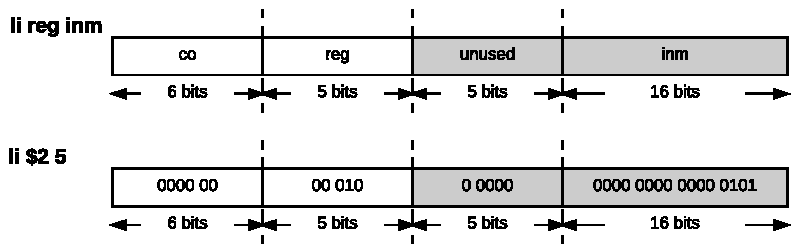
\includegraphics[width=14cm]{figures/instruction_example_traduction}
 	\caption{Formato de instrucción descrito en el \gls{microcodigo} y ejemplo de su traducción en binario.}
	\label{fig:software_assembly_traduction}
\end{figure}

Una de las grandes ventajas del simulador \acrshort{wepsim} es que no está limitado a un conjunto de instrucciones concreto. Se puede definir un amplio conjunto de instrucciones de procesadores reales o inventados. Se puede usar para añadir por ejemplo, a un conjunto de instrucciones MIPS, otras instrucciones diferentes no incluidas en dicho conjunto de instrucciones.

\subsection{Kernel del simulador}
\label{sec:kernel_simulator}

El kernel del simulador, es el componente que integra la interfaz de usuario del simulador, el controlador del simulador, y el motor de simulación, siendo el encargado de hacer las funciones de controlador de la herramienta gestionando las comunicaciones de la interfaz de usuario con los modelos \gls{hardware} y \gls{software}. 

De esta forma cuando el usuario interacciona con la interfaz gráfica, el módulo encargado de la interfaz genera eventos que identifican las acciones que el usuario realiza. Estos eventos son generados a modo de peticiones al controlador de la simulación, que se encarga de identificar el evento generado, comprobar el contexto en el cual se encuentra, y enviar la acción correspondiente a realizar al motor del simulador. El motor del simulador, se encarga de comunicarse con los modelos \gls{hardware} y \gls{software}, de forma que estos puedan ejecutar correctamente la acción solicitada (Figura \ref{fig:kernel_diagram}).

\begin{figure}[htbp]
 	\centering
 	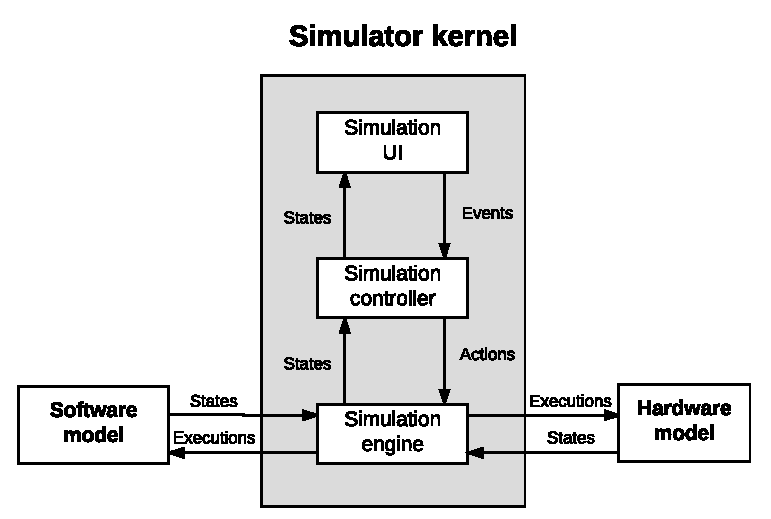
\includegraphics[width=10cm]{figures/kernel_diagram}
 	\caption{Arquitectura del kernel del simulador.}
	\label{fig:kernel_diagram}
\end{figure}

Por ejemplo, si el usuario selecciona la ejecución de un ciclo de reloj, la interfaz de usuario genera el evento correspondiente. El controlador del simulador, se encarga de identificar el evento, verificar que se cumplen todas las condiciones para poder ejecutarse un ciclo de reloj comprobando diferentes valores del estado del simulador. En caso de poder ser realizada la ejecución del ciclo de reloj, envía la orden al motor del simulador que se encarga de comunicarse con el  modelo \gls{hardware}, realizando la ejecución de un ciclo de reloj actualizando los componentes del modelo \gls{hardware}. Por último, la interfaz de usuario consulta el estado del modelo \gls{hardware} actualizando la información necesaria para ser mostrada al usuario.




